\documentclass[12pt,a4paper]{report}

% Packages
\usepackage[utf8]{inputenc}
\usepackage[T1]{fontenc}
\usepackage{geometry}
\usepackage{tikz}
\usetikzlibrary{arrows, positioning, shapes, fit}
\usepackage{float}

% Page setup
\geometry{a4paper, margin=1in}

% Title
\title{Test Diagrams for Campus-Sync Report}
\author{Mausam Kar}
\date{\today}

\begin{document}

\maketitle

\chapter{Test Diagram}

\section{Simple Test Diagram}

\begin{figure}[H]
    \centering
    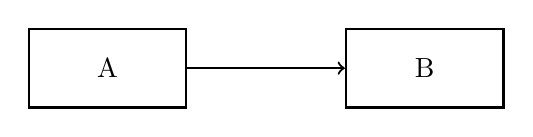
\begin{tikzpicture}[thick, node distance=2cm]
        \node (A) [draw, rectangle, minimum width=2cm, minimum height=1cm] {A};
        \node (B) [draw, rectangle, minimum width=2cm, minimum height=1cm, right=of A] {B};
        \draw[->] (A) -- (B);
    \end{tikzpicture}
    \caption{Simple test diagram}
\end{figure}

\end{document}